
\section{Simulation}
Accurate and efficient simulation is a critical component of this project, as the study of adaptive containment strategies for epidemics in metapopulation networks relies on robust numerical methods. The underlying system of ODEs demands precise integration schemes to capture both quantitative and qualitative dynamics accurately. Simultaneously, the large size of the networks and the need for ensemble simulations require computationally efficient algorithms and data structures.\\

This chapter outlines the numerical methods employed to analyze the system's dynamics across various configurations and network structures. It includes a discussion of the tools, data structures, numerical solvers, data processing, and visualization techniques used. Special attention is given to the integration schemes, as trivial methods necessitate impractically small time steps to maintain accuracy, leading to poor performance and significant errors. Improved solvers were implemented to achieve better error scaling with respect to the time step.\\

Furthermore, efficient data structures and algorithms were developed to address scaling challenges posed by large networks. This requirement was amplified by multi-step integration schemes, which necessitate managing multiple concurrent states of the network. The combined focus on accuracy and efficiency ensures that the simulations can effectively support the analysis of adaptive epidemic containment strategies.\\

\subsection{ODE System Properties}
When solving an ODE, it is critical to first understand its type and properties, as different require different integration or solver schemes. The entire system of ODE system is represented in the set of infection dynamics and travel restriction equations. Although the system of ODEs is not time-dependent, it is still of-interest to keep accurate record of the elapsed time as the state of the system changes, as the main focus of this study is to find the spread rate of infection in the system, which requires knowledge of when different populations hit their infection peak. 
\\

Based on the design of the model, it is expected that at all times, the sum of all compartments of individuals in all subpopulations should remain constant. Furthermore, due to the formulation of the mobility rates between subpopulations, it is expected that the total number of individuals at each subpopulation is also conserved. \\

There are many possible cases in which the ODE becomes stiff. Stiff ODEs are ones in which different variables change on different timescales. In the case of this model, possible cases include: Infection rates are much faster than recovery rates, the mobility matrix $\Delta$ has very different time scales, and population sizes vary significantly between subpopulations. However, with somewhat realisitic model parameters, these disparagements do not cause significant stiffness. The two major sources of stiffness that can be found in the ODE and have been observed in the numerical simulation are:
\begin{itemize}
	\item \textbf{Fast infection spread in the wavefront:} In both the adaptive and non-adaptive system, it is found that the infection spreads in wave at a somewhat constant speed. This wave is characterized by consecutive rapid spread of infection in subpopulations based on how far away in the network from the initial infection. This causes step-wise process where at any point in time a small group of the metapopulation having very rapid internal spread of infection while the remainder of the subpopulations have already been infected or are yet to be sufficiently infected. This translates to wildly different rates of change number of infecteds in the different metapopulations, which contributes stiffness to the system.
	\item \textbf{Fast travel restriction in the wavefront:} In the adaptive system, it was found that the proportionality constant for the  travel restriction, $\lambda$, needs to be sufficiently high to have an effective slow-down of the infection spread across the network. However, this causes travel restriction to change on a much faster than the infection variables especially around the wavefront. This adds another source of stiffness to the model. 
    
\end{itemize}

Based on the structure of the ODE, one can also prove that the solution should lie within a certain system domain which it is unable to escape. Examples of boudaries of this manifold include the size of any infection compartment becoming negative or surpassing the total subpopulation size, and travel restrictions being restricted in the range from 0 to 1. Besides the fact that a numerical solution exceding these boundaries is an obvious sign that the integration scheme is erroneous, exiting this domain could result in numerical oscillations or even divergence from the solution entirely. An example of this is travel restriction turning negative which would result in it having a negative rate of change, causing exponential growth in the negative direction.\\

There are several sources of nonlinearity in this system of ODEs, such as the $S_{x} I_{x}$ term in infection spread, and $\bar \rho I_{x}$ in travel restriction. Nonlinear terms can lead to numerical instabilities, exacerbate error propagation, among other things. Simple integration schemes that do not take into consideration accuracy and stability would be prone to errors. Furthermore, nonlinear systems often require iterative solvers for implicit methods, increasing computational cost, especially with large-scale systems.\\

It is also worth to keep in mind the level of sparsity in the adjacency matrix as it impacts the expected scaling of computational cost with network size. With sufficienty large matrices, it can be expected that the total computation time will asymptotically approach the scaling of number of links in the network, For sparse and scale-free networks, this scaling can be close to linear, causing little concern for computational cost scaling with large networks.\\

However, another trait of the topology, the degree distribution, also plays a role in the computational cost. In particular, parallelizability of the code can suffer significantly from work imbalance. Since the numerical integrator iterates over nodes, and not links, it is sensetive to the heterogeniety of the degree distribution. For example, in scale-free networks, highly connected nodes (called hubs) can have orders of magnitude more links than the nodes on the perefery. This heterogeniety can make parallizing the code, where each process or thread finds the rate of change for only a select group of nodes, have imbalanced work distribution, possibly slowing down the computation to the worst-case-scenario for a single thread. This can be at least partially remedied by finding a mapping that minimizes the total number of links each thread is responsible for, which is by itself a non-trivial problem.\\

Another property of the ODE to take into consideration is high variance in rates of change as this causes huge inefficiencies in computation if inappropriate solvers are used. It can be observed that given the non-zero initial condition of the number of infecteds of the first infected subpopulation. Due to the required high value of $\lambda$, initial growth of the immediate neighbors of the infected subpopulation can have arbitrarily high growth rate of the travel restriction. This is in contrast to the much lower rates of change for all subsequently infected subpopulations, as they react to incoming infecteds that start and grow continuously from an initial condition of zero infected.\\


\subsection{Numerical Simulation}
\subsubsection{Language and Tools}
The Julia programming language was used for the computational aspect of this project. The main known advantage of Julia is its out-of-the-box speed in scientific computation due to its  Just-in-time compiler. This gives a head-start in computational speed compared to C++ and Python which require significantly more complex setups. However, Julia has several other positive aspects that make it especially useful for this project. This includes its strong variable typing, multiple dispatch, and strong support for functional programming. It also incorporates many mathematical tools dealing with matrix operations and numerical equations. For dealing with networks, Graphs.jl was used for generating network classes, such as the Barabasi-Albert and the Watts-Strogatz networks, and for typical graph functionality such as finding path length and nearest neighbors. Karnak.jl was used for network visualization and Plots.jl was used for all the plots in this report.
\subsubsection{Data Structure}
In designing an efficient and scalable data pipeline for epidemic simulations, the choice of data structures plays a critical role. These structures must support both static and dynamic components of the simulation while ensuring memory efficiency and computational speed. This subsection delves into the underlying principles guiding these choices, such as the use of structs, the importance of memory contiguity, and the modularization of code for optimizing computational performance.\\

\begin{figure}
	\centering
	\includegraphics[width=120mm]{Figures/structs code.png}
	\caption{\small Modular struct structure of a metapopulation}
\end{figure}

The aspect that taken under consideration the most in the data structure is Memory contiguity, which refers to the arrangement of data in sequential memory locations. This is important because modern computer architectures leverage caching mechanisms to speed up data retrieval. Contiguous memory allows processors to fetch adjacent data elements in fewer operations, significantly boosting performance for tasks that iterate over large datasets. For epidemic simulations, where data structures like adjacency matrices and population compartments are frequently accessed, maintaining memory contiguity minimizes latency and ensures efficient computational workflows.\\

The struct (short for structure) was used extensively in this project. It is a user-defined composite data type that groups related variables under a single name, allowing them to be accessed and managed as a unit. They play a more bare-bones analog to classes in object-oriented programming. Structs enhance readability, ensure logical grouping, and facilitate passing complex data efficiently between functions while reducing the risk of accidental modifications. However, the most crucial benefit of structs is that they can be static, immutable and of preallocated size. This allows for great compiler optimizations as the reading and writing processes can be streamlined.\\

\begin{figure}
	\centering
	\includegraphics[width=120mm]{Figures/Population RoC code.png}
	\caption{\small Computation of the rate of change of a subpopulation}
\end{figure}
The usage of structs allows for Modularization in code design, which ensures that computational tasks are divided into smaller, self-contained functions or modules. For epidemic simulations, modularization allows dynamic operations—such as updating epidemiological states or applying travel restrictions—to be isolated within specific functions. These contained spaces reduce the scope of local variables and ensure that memory access patterns remain predictable, leading to optimized resource utilization. Additionally, modularization promotes parallel development and debugging by isolating distinct computational aspects into manageable units.\\

There are two types of data in this sytem: 
\begin{itemize}
	\item The static parameters and properties of the metapopulation, such as the mobility rate and link weights.The static parameters were stored in a collection of immutable structs such as epidemic and network properties. This grouping allows for safe and efficient passing of constants to functions. It's worthy to note that while there is different link weights between nodes, the network overall is still sparse such that the majority of links between any two nodes are zero-valued.
	\item The dynamic data such as the number of infected individuals in each subpopulation and travel restrictions which change with time. The dynamic variables in this system all happen locally in relation to the subpopulations. The two aspects of these dynamics for any given subpopulation are the sizes of the different epidemiological states and the travel restrictions applied towards all of its neighbors. These dynamic data were stored in structs representing each subpopulation. These include the population compartmental variables and the travel restricitions applied by the subpopulation towards all neighboring populations.
\end{itemize}

The utilization of structs came in especially useful when implementing multistep integration schemes. Since they require the multiplication and scaling of the system at different timesteps, special definitions for scaling and adding metapopulations are needed. Julia's multi-dispatch was utilized here for streamlined manipulation of system variables. In addition to struct definions of the system itself, a special struct was defined that stores the rate of change of each subpopulation as well.\\

The graph structure is stored in the form of a sparse weighted adjacency matrix in the form of a Compressed Sparse Column (CSC).  CSC is composed of 3 arrays of element values, row indices array and column pointers array. CSC was chosed and not Compressed Sparse Row, because Julia is column-major. The storage size of this format is linearly proportional to the number of elements in the adjacency matrix and hence to the network link density. Even though this matrix is symmetrical and thus would only require the storage of the lower rectangular region, the entire matrix is stored with both its symmetric sides. This is to improve the retrieval time to attain the indices of neighboring subpopulations. In a CSC adjacency matrix, values in each column are stored contiguously, and hence are quick to read from memory. However, to maintain this advantage, each column has to be fully stored so that each subpopulation can quickly find all its neighbors.\\
\usetikzlibrary{matrix}
\usetikzlibrary{positioning}
\begin{figure}[htbp]
	\centering
	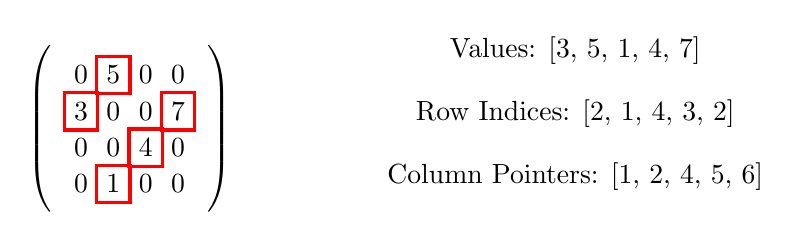
\begin{tikzpicture}
	  % Draw the sparse matrix
	  \matrix[matrix of math nodes, left delimiter={(}, right delimiter={)}] (A)
	  {
		0 & 5 & 0 & 0 \\
		3 & 0 & 0 & 7 \\
		0 & 0 & 4 & 0 \\
		0 & 1 & 0 & 0 \\
	  };
	
	  % Highlight non-zero elements
	  \foreach \i/\j in {2/1,1/2,4/2,3/3,2/4} {
		\draw[red, very thick] (A-\i-\j.north west) rectangle (A-\i-\j.south east);
	  }
	
	  % Draw arrays for CSC representation
	  % Values array
	  \node[right=3cm of A, yshift=1cm] (values) {Values: [3, 5, 1, 4, 7]};
	  % Row Indices array
	  \node[below=0.2cm of values] (row_indices) {Row Indices: [2, 1, 4, 3, 2]};
	  % Column Pointers array
	  \node[below=0.2cm of row_indices] (col_pointers) {Column Pointers: [1, 2, 4, 5, 6]};
	
	  % Arrows from matrix to Values array
	%   \draw[->] (A-2-1) to[out=0,in=180] (values.west);
	%   \draw[->] (A-1-2) to[out=0,in=180] (values.west);
	%   \draw[->] (A-4-2) to[out=0,in=180] (values.west);
	%   \draw[->] (A-3-3) to[out=0,in=180] (values.west);
	%   \draw[->] (A-2-4) to[out=0,in=180] (values.west);
	\end{tikzpicture}

	\caption{Illustration of Compressed Sparse Column (CSC) storage format. Sparse one-dimensional arrays are stored in a similar manner except without the need for column pointers.}
	\end{figure}

Following the simulation, we are interested in the history of all the dynamic variables. One could store an array copies of the metapopulation, one for each time iteration. However, this data structure would have poor data contiguency. As in the data analysis we will mostly process each variable independently (e.g. looking at the evolution of infected in each subpopulation). Instead, seperate arrays for each of the variables were assigned and appended to with every time step. For the travel restrictions, an array of sparse matrices was stored, where each matrix is the travel restrictions applied from every subpopulation to every other subpopulation. This has the disadvantage that when looking solely on travel restrictions between two subpopulations over time, there is a relatively large span between consecutive time values. However, it was found that reordering the data structure to be a sparse matrix of arrays (where each element is the travel restriction history of a pair of subpopulations) took more time to create than just reading from the array of sparse matrices.\\


\subsubsection{Integration Scheme}

Selecting an appropriate integration scheme is vital for accurately solving the system of ODEs governing the epidemic dynamics and adaptive travel restrictions. Initially, the Explicit Euler method was employed due to its simplicity. However, it required impractically small time steps to maintain stability and accuracy, especially in the presence of stiffness and nonlinearities in the system.\\

To improve accuracy without significantly increasing computational complexity, the classical fourth-order Runge-Kutta (RK4) method was implemented. The RK4 method provides a good balance between computational efficiency and accuracy by calculating intermediate stages within each time step to achieve fourth-order accuracy. The implementation of RK4 for advancing the solution from time $t$ to ( $t + \Delta t$ ) is as follows:

\begin{align*} 
	k_1 &= f\left(y_t,, t\right), \\ k_2 &= f\left(y_t + \tfrac{1}{2}\Delta t, k_1,, t + \tfrac{1}{2}\Delta t\right), \\ k_3 &= f\left(y_t + \tfrac{1}{2}\Delta t, k_2,, t + \tfrac{1}{2}\Delta t\right), \\ k_4 &= f\left(y_t + \Delta t, k_3,, t + \Delta t\right), \\ y_{t + \Delta t} &= y_t + \tfrac{1}{6}\Delta t\left(k_1 + 2k_2 + 2k_3 + k_4\right), \end{align*}

where $y_t$ is the state vector at time $t$, and $f$ represents the ODE system.

Despite the improvements, the RK4 method still faced challenges with stiffness and ensuring that dynamic variables remained within their realistic bounds (e.g., compartment sizes staying non-negative and not exceeding total population sizes). To address these issues, an adaptive Runge-Kutta-Fehlberg RK4(5) method with adaptive time stepping was implemented.

The RK4(5) method dynamically adjusts the time step based on:
\begin{itemize}
	\item \textbf{The estimated local truncation error:} Allowing for efficient handling of varying timescales in the system. This adaptivity enables larger time steps when the solution changes slowly and smaller steps during rapid transitions, improving computational efficiency without compromising accuracy.
	\item \textbf{Existance within the solution domain.} Since the system has very clear-cut boundaries of the system variables, it is easy to check when any one steps beyond its theoretical limit. Simply reducing the step size until no variable steps out-of-bound was sufficient. The checks were not only done at each integration step but each individual derivative evaluation, to eliminate errroneous derivative contribution to the integration step.
\end{itemize}  

By employing the adaptive RK4(5) method, the simulation effectively balances accuracy and efficiency, handling stiffness in the ODE system while maintaining the physical realism of the solution throughout the simulation.


\subsubsection{Visualization}
Typically, visualizing dynamics on networks and especially dynamics of network without animation can be quite challenging, as there is a lot of temporal information that needs to be conveyed in a single or a few still graphs. However, certain dynamical invariances can be made use of to reduce the amount of information that can communicated the temporal information. In this case, it has been observed that the evolution of the SIR compartmental sizes all follow a nearly-identical trajectory, at least in linear space (which is typically the one of interest in decision making), where the only major difference is the time offset of this trajectory. The objective is now to clearly communicated the time (in days) at which each subpopulation hit its peak infection day, as it is the date of most interest (showing the date at which the subpopulation hit the infected fraction equivalent to $i_0$ would also work). The same logic could also be applied to the travel restriction dynamics, where instead we're interested in showing the date at which full travel restriction was implemented. The kamada kawai layout was used to compute the network layout. 

\begin{figure}[!ht]
    \centering
    \includegraphics[width=120mm]{Figures/Network_β0.25_γ0.05_σ0.0_μ0.01_nPop25_kbar4_topologySmallWorld_λ0.0_mobBias0.0_h0.1_minh1.0e-9_nDays1000_I01.0e-5_critRange0.0.pdf}
    \caption{\small Network visualization of a Barabasi-Albert network with number of added links per node ($m$) is two links. Indices show the day at which each population has reached its peak infection fraction. The subpopulation with initial condition infection is marked in red.}
    \label{}
\end{figure}

\begin{figure}[!ht]
	\centering
	\begin{minipage}[b]{0.45\textwidth}
		\includegraphics[width=\textwidth]{Figures/Animation Frame 1.png}
	\end{minipage}
	\hfill
	\begin{minipage}[b]{0.45\textwidth}
		\includegraphics[width=\textwidth]{Figures/Animation Frame 2.png}
	\end{minipage}
	\vfill
	\begin{minipage}[b]{0.45\textwidth}
		\includegraphics[width=\textwidth]{Figures/Animation Frame 3.png}
	\end{minipage}
	\hfill
	\begin{minipage}[b]{0.45\textwidth}
		\includegraphics[width=\textwidth]{Figures/Animation Frame 4.png}
	\end{minipage}
	\caption{Animation frames showing the progression of the epidemic over time in a Watts-Strogatz network. The system is Susceptible-Infected-Recovered (Blue, Red, Green) compartmental system with connection proportional response strategy with no mobility restoration bias. The animation shows the state of the system at the initial condition of the system (the black-bordered patch is the subpopulation with an initial small infected fraction). Over time, the infection starts spreading within the first subpopulation along with its near neighbors. The flow rate of infected individuals across connections can be seen by the red tinting of connections. Along with the spread of the infection, many subpopulations start to increase their travel restriction to even mildly-infected patches which can be seen by the low or no opacity of some link endpoints. Over time, eventually the infection to spreads substantially to the rest of the network while many subpopulations nearly recover. In the final state of the metapopulation network, all populations have negligible amount of infected while the vast majority are recovered individuals.}
\end{figure}

\clearpage
\subsection{Simulation Results}

Besides the numerical simulations done to confirm the findings in the Analysis chapter, further simulations were done to observe the behavior of the described metapopulation networks in both nonadaptive and adaptive configurations with the proposed travel restriction strategies. Unlike what was shown in the analysis, however, there is a need here for network topologies that reflect transportation networks as seen in real life. The two main aspects that are desirable to be captured are clustering and small-world traits. Clustering is when nodes have a tendency to form triangles with their neighbors, while small-worldness is when the average path length between any two nodes is small compared to the number of nodes in the network. Two network topologies which have these traits that were used as a testbed: undirected unweighted Watts-Strogatz (Small World) and Barabasi-Albert (Scale-free) networks % REF
, which have an average number of links per node $\bar k=4$ unless stated otherwise.\\

To test the heterogeneous diffusion model described in chapter 2 and to better reflect real world distributions, a random subpopulation size distribution that is exponentially distributed (with an average of 1) was applied for some of the case scenarios. Although there is an observed relationship between population size and its connectivity, no such correlation was applied here for simplicity. For similar reasons, the exponential distribution was chosen instead of a power-law distiribution. %REF
However, due to the fundamentally stochastic nature of the chosen network topologies, the randomness of a randomly generated network could introduce biases to a simulation. To remedy this, ensemble simulations were sometimes done such that a group of several different networks, of the same topology and traits, with but different random number generator seeds, were simulated together. Aggregation and averaging was then taken for the parameters of interest and in some cases all ensemble results were shown. The size of the ensemble was made large enough until it was observed there was negligible change in the output range. To start a case scenario, a randomly selected subpopulation is chosen and whose infected subpopulation is set to the value $I_j=i_0$.\\ 

\subsubsection{Spread Rate in clustered networks}
Since the analysis done in chapter 3 was only done on a 1-lattice, which is not representative of real-world network, it is important to see if the findings from it are at least partially applicable to more realistic networks, especially ones with higher clustering. To compare, we start with the non-adaptive model and see if the Lambert W function approximation, expressed in equation \ref{eq: Lambert W approximation}, is valid for other network topologies. A Watts-Strogatz network of size 50 subpopulations was used with $\bar k=4$, rewiring probability = 0.5, $\beta=0.25,\gamma=0.05,\mu=0.01,i_0=10^{-5}$.\\

The finding from the analysis was that in the non-adaptive system, there is a constant spread rate of infection throughout the network such that the initial infection day ($t_j=i_0$) is linearly proportional to the path length $j$. It was also found that this relationship applies to the peak infection day. Simulation was done to see if the same relationship applies for a Watts-Strogatz network. The results can be seen in figure \ref{fig: Watts Strogatz spread days path lengths and resistance distances} (a).As expected, there was found to be some variation for the infection spread time and peak infection time as a function of the path length distance. This is because the path length alone doesn't give the full picture the different paths infected individuals can migrate to it. However, it was found that the variance wasn't very high. Of course, this variance is expected to differ based on the topology and other epidemic parameters. Furthermore, it can be seen that the linear relationship between infection day and path length is still mostly preserved. An even more surprising finding is that the Lambert W approximation in equation \ref{eq: Lambert W approximation} is quite to the average spread rate in the network. This is true to a lesser extent for the peak infection day, where it is observed that they somewhat convergance more to each other such that they're not as spread out over time as the initial spread time.\\

To solve the issue of path length not being representative, a different distance measure was tested, as discussed in section 3.3. It was desirable to choose a distance measure that's easy to compute but one that takes into consideration the diffisive nature of the metapopulation network. The resistance distance, which is computed through the pseudoinverse of the signed Laplacian matrix, was used\cite{xiao2003resistance}. The value of the resistance distance measure is the same as the path graph in a 1-lattice but can be lower in a clustered matrix like Watts Strogatz. The measure was found to give a better representative mean of spread infection date but with the cost of having wider variance. Alternative distance measures should be tested to check for different network topologies and confirmed with numerical testing.

\begin{figure}[!ht]
	\centering
	\begin{minipage}[b]{0.45\textwidth}
		\includegraphics[width=\textwidth]{Figures/Spread and Peak Infection Days (pathLengths)_β0.25_γ0.05_σ0.0_μ0.01_nPop50_kbar4_topologySmallWorld_λ0.0_mobBias0.0_h0.1_minh1.0e-9_nDays1000_I01.0e-5_critRange0.0 CUSTOM.pdf}
		\centering
		(a)
	\end{minipage}
	\hfill
	\begin{minipage}[b]{0.45\textwidth}
		\includegraphics[width=\textwidth]{Figures/Spread and Peak Infection Days (resistance_distances)_β0.25_γ0.05_σ0.0_μ0.01_nPop50_kbar4_topologySmallWorld_λ0.0_mobBias0.0_h0.1_minh1.0e-9_nDays1000_I01.0e-5_critRange0.0 CUSTOM.pdf}
		\centering
		(b)
	\end{minipage}
	\caption{\small Spread infection days and peak infection days in a Small-World network vs different distance measures from the initially-infected subpopulation compared with the Lambert W expected spread rate. Figure (a) shows the path length (number of consecutive jumps over connections). The plot shows some variance at each path length and has a slightly higher slope than the Lambert W approximation. Figure (b) uses the resistance distance measure which evaluates to a real number that is much lower value. The relationship between spread infection and distance is more scattered than the path length. However, the Lambert W is a better approximation here. It can also be seen that the peak infection days maintain the linear dependence but with a slightly flatter slope. }
	\label{fig: Watts Strogatz spread days path lengths and resistance distances}
\end{figure}

However, even in a network that is low in clustering, it is important to realize the impact of the node degree distribution and dimensionality of the network on how quickly the infection spreads across the global population inhabiting all patches. For example, in a 2-lattice (a cartesian grid of patches) the number of patches at any given path length is linearly proportional to the path length itself. That means that for a constant spread rate of infection as defined for the 1-lattice, the total number of infected individuals grows quadratically as time goes on. For Scale-free networks, the scaling can be much higher than that. Hence, it is important to take into account the dimensionality of the network to predict the peak concurrant infected over time and impact of travel restrictions.

\begin{figure}[!ht]
	\centering
	\begin{minipage}[b]{0.45\textwidth}
		\includegraphics[width=\textwidth]{Figures/Prevalence of Infected_β0.25_γ0.02_σ0.0_μ0.01_nPop50_kbar3_topologySmallWorld_λ0.0_mobBias0.5_h0.1_minh0.01_nDays1000_I01.0e-5_critRange0.0 CUSTOM.pdf}
		\centering
		(a)
	\end{minipage}
	\hfill
	\begin{minipage}[b]{0.45\textwidth}
		\includegraphics[width=\textwidth]{Figures/Prevalence of Infected (Ensemble)_β0.25_γ0.02_σ0.0_μ0.01_nPop25_kbar3_topologySmallWorld_λ0.0_mobBias0.5_h0.1_minh0.01_nDays1000_I01.0e-5_critRange0.0 Custom.pdf}
		\centering
		(b)
	\end{minipage}
	\caption{\small  (a) The cumulative size of infected individuals in a non-adaptive SIR Watts-Strogatz metapopulation network of size 50. Figure (b) is an ensemble simulation of 20 random Watts Strogatz network that shows the total infected size. While there are network-based variance in the evolution of infected size (as the number of individuals at varying distances can change from one network to the other), a single peaked average was found in the ensemble simulation.}
	\label{fig:Infected-Evolution-cumu-and-ensemble}
\end{figure}

\subsubsection{Adative strategies}

With the code structure being modular, it is easy to implement different travel restriction strategies and see how they impact the mobility network. Of particular interest is the infection spread rate, as the primary role of travel restriction is to slow down or to "flatten the curve" of the total global infectected count. All 4 travel restriction strategies (as described in section 2.3) along with the non-adaptive strategy, are tested first on a finite 1-lattice to see clearly how they perform with no clustering. For the three linearly proportional strategies, $\lambda=10^7$, while for the logarithmic strategy, a value of $\lambda = 0.1$ was choses and an $I_{min}=10^{-10}$.  All other traits and parameters are the same as given in this section. We start in this subsection with the strategies without mobility restoration bias. \\

\begin{figure}
    \includegraphics[width=\textwidth]{Figures/Spread Infection Days different strategies_β0.25_γ0.0_σ0.0_μ0.01_nPop10_kbar4_topologyPathGraph_λ0.1_mobBias0.0_h0.1_minh0.01_nDays1000_I01.0e-5_critRange0.0.pdf}
    \caption{Spread infection days for different strategies: No restriction, Global proportional restriction, Uniform proportional restriction, Connection proportional restriction, and Connection logarithm restriction. The No restriction and Connection-proportional restriction show similar patterns as previously analyzed, with a steady spread rate. The Uniform proportional restriction shows a delay in infection spread for subpopulations 2 and 3. The Global restriction maintains a slowed spread rate across the network. The Connection-logarithm restriction shows promise in slowing the spread rate for a sizable distance around the initially infected subpopulation.}
    \label{fig:spread-day-strategies}
\end{figure}

As seen in Figure \ref{fig:spread-day-strategies}, the No restriction and Connection-proportional restriction are as previously found in the analysis section. For the Uniform proportional travel restriction, we find a somewhat similar result to the connection based one, where instead of a slowdown happening for only the immediate neighbor of the initially infected subpopulation, the subsequent one also takes a longer time to get infected. Though it is not as easy to understand why analytically (because this strategy doesn't have the locality found in the connection-based strategy), there is a satisfactory explanation of why this is the case from the understanding of the previous analysis. Due to the fact that the when subpopulation 2 restricts incoming traffic from subpopulation 1, it also restricts the outflow of individuals going to subpopulation 3, since in the Uniform strategy $\rho_{2,1}=\rho_{2,3}=\rho_2$, which is goverened by the relationship

$$
	\dot{\rho}_2=\lambda M_{(I);2}= \lambda \mu (\bar{\rho}_{1} \bar{\rho}_{2} I_1 + \bar{\rho}_{2} \bar{\rho}_{3} I_3) \approx \lambda \mu \bar{\rho}_{1} \bar{\rho}_{2} I_1,
$$

which approximately equals $\dot{\rho}_{2,1}$ in the connection proportional strategy. $\rho_2$, in turn, affects $M_{(I);3}$ the same way to cause a delay in spread infection day $t_3$. And for similar reasons, the spread rate falls to the non-adaptive spread rate after that.\\

The Global travel restriction also behaves the same way for the first three subpopulations, but manages to maintain this slowed down spread rate for the rest of the network. This is because the whole network, even in connections between relatively healthy subpopulations, are restricted in the same manner as the ones near the initially infected subpopulation. This slowed-down spread rate was found to hold true even for large networks.The fact that the same spread rate is maintained for all three strategies is due to the formulation of strategy formulas to let $\lambda$ have the same impact on travel restriction given the same infected mobility flow.\\

\begin{figure}
	\centering
    \includegraphics[width=100mm]{Figures/Evolution of Path Mobility Restrictions_β0.25_γ0.0_σ0.0_μ0.01_nPop10_kbar4_topologyPathGraph_λ0.05_mobBias0.0_h0.1_minh0.01_nDays1000_I01.0e-5_critRange0.0.pdf}
    \caption{\small The different downstream applied restrictions in an SI system on a path graph with a Connection logarithm strategy. It can be seen that they start with an immediate high slope and then taper off to a value of 1 or somewhat below that. Unlike the other proportional strategies, here the order of starting or finishishing restricting traffic does not necissarily follow the path length distance from the initially infected subpopulation.}
    \label{fig:log-Restriction}
\end{figure}

Finally, the Connection-logarithm travel restriction strategy was the only local strategy that showed the most promise in slowing down the infection spread rate for a sizable distance around the initially infected subpopulation. The dependence on the ratio between incoming infected vs local infection growth (as defined by $\dot{\rho}_{xx'} = \lambda \log\left(\frac{\kappa I_{x} + M_{(I);x,x'}}{\kappa I_{x}}\right)$), allowed for far away subpopulation to react early to signs of infection spread. In the case of an unconstrained measurement of both local and incoming infected ($I_{min}=0$), it was found that the spread rate converges to that acheived by the global strategy. Since, however, such a value would be unrealistic (and result in infinite growth around $I_x=0$), we are more interested in the scenario where $I_{min}>0$, which diminishes the effect of the strategy for far away patches. It was found that while attaining a slowed down effect for several patches at a far away distance, it eventually collapses to the non-adaptive spread rate. The width of the region of slowed down spread rate is proportional to $log(1/I_{min})$.\\

It is important to note as well the behavior of the travel restriction applied in the Connection Logarithm strategy, as it differs in behaviour from the other ones. While the proportional strategies, given the incoming infected flow start smoothly from zero, the applied travel restriction also starts from zero. They also eventually reach the maximum restriction value 1. On the other hand, due to the usage of the ratio of incoming infected vs local growth, there is an instantaneous nonzero slope as soon as $I_x>I_{min}$ which starts decreasing as the internal growth outpaces the incoming flow. In fact, $\dot \rho$ can decrease fast enough to not actually reach a value of 1 before , as the ratio becomes dominated by the internal growth. This has the nice benefit of maintaining some network activity while slowing down the spread. However, an unrealistic outcome of this strategy is that there is a tendency of populations which are detecting small amounts of inflow can react more severely than ones that are right next to the initially infected subpopulation. This issue could be solved by introducing a hybrid strategy that takes into consideration both the absolute value and the ratio. 

\subsubsection{Mobility restoration}
\begin{figure}[!ht]
	\centering
	\begin{minipage}[b]{0.45\textwidth}
		\includegraphics[width=\textwidth]{Figures/Evolution of Path Mobility Restrictions_β0.25_γ0.02_σ0.0_μ0.01_nPop10_kbar3_topologyPathGraph_λ10000.0_mobBias0.0_h0.1_minh0.01_nDays1000_I01.0e-5_critRange0.0.pdf}
		\centering
		(a)
	\end{minipage}
	\hfill
	\begin{minipage}[b]{0.45\textwidth}
		\includegraphics[width=\textwidth]{Figures/Evolution of Path Mobility Restrictions_β0.25_γ0.02_σ0.0_μ0.01_nPop10_kbar3_topologyPathGraph_λ10000.0_mobBias2.0_h0.1_minh0.01_nDays1000_I01.0e-5_critRange0.0.pdf}
		\centering
		(b)
	\end{minipage}
	\caption{\small (a) The applied travel restrictions in a 1-lattice with no mobility restoration bias, showing a quick shutdown of the network as restrictions remain in place even after infection subsides. (b) The applied travel restrictions with mobility restoration bias, demonstrating a decrease in restrictions as the infected flow lowers, eventually reaching zero when the infection wave has terminated.}	\label{fig:Evolution-Restriction-without-and-with-bias}
\end{figure}

Finally, we take a look at the impact these travel restrictions have had on the network activity. As previously discussed, it is expected that, without some kind of mobility restoration mechanism, in an SIR model, the network quickly shuts down as travel restrictions are applied against any population that has been infected. Even after infection has subsided, the restrictions are still in place. For this reason, a mobility restoration bias $b$ was introduced in the different strategies (as seen in equations 2.29 to 2.32). As found in the modeling section, after the initial rise of travel restrictions due to infected mobility, and then the source of infected flow start to recover and cause the composition of incoming flow to have less infected, travel restrictions start to decrease due to the mobility restoration bias. An equilibrium is between the inclination of $\rho$ to increase due to the existing incoming infected and the mobility bias. This equilibrium gets lower as the infected flow lowers and reaches zero when the infection wave has terminated. This behavior can be seen in Figure \ref{fig:Evolution-Restriction-without-and-with-bias} (b).\\

The net effect of having this mobility bias is enabling the restoration of network activity following an SIR type wave. The formulation of the bias in the travel restriction strategies, given a sufficiently small bias, causes diminished impact on subpopulations facing a large influx of infected (which can be inferred by the fact that most travel restrictions are able to reach a value of 1 during the peak infected flow) while cutting back on restrictions when there is little relevance to the infection spread dynamics. This causes a net effect of a total restoration of mobility not long after the infection in the metapopulation has subsided, as can be seen in Figure \ref{fig:Mobility-flow-without-and-with-bias}

\begin{figure}[!ht]
	\centering
	\begin{minipage}[b]{0.45\textwidth}
		\includegraphics[width=\textwidth]{Figures/Cumulative Mobility Flow_β0.25_γ0.02_σ0.0_μ0.01_nPop50_kbar3_topologySmallWorld_λ10000.0_mobBias0.0_h0.1_minh0.01_nDays1000_I01.0e-5_critRange0.0.pdf}
		\centering
		(a)
	\end{minipage}
	\hfill
	\begin{minipage}[b]{0.45\textwidth}
		\includegraphics[width=\textwidth]{Figures/Cumulative Mobility Flow_β0.25_γ0.02_σ0.0_μ0.01_nPop50_kbar3_topologySmallWorld_λ10000.0_mobBias2.0_h0.1_minh0.01_nDays1000_I01.0e-5_critRange0.0.pdf}
		\centering
		(b)
	\end{minipage}
	\caption{\small Cumulative network mobility across the network without bias (a), showing a prolonged shutdown even after infection subsides, and with bias (b), demonstrating a gradual restoration of mobility as the infected flow decreases, eventually reaching normal levels when the infection wave has terminated.}	\label{fig:Mobility-flow-without-and-with-bias}
\end{figure}

